\section*{RESULTS}\label{results}
\subsection*{Roll decay model tests}\label{roll-decay-model-tests}
\subsubsection*{Test at 0 knots}\label{test-at-0-knots}
Two roll decay model tests were conducted at zero speed referred to as
Run 1 and 2 \citep{7505983/5DP3HN8F}.
These tests where analyzed by fitting a quadratic model
to the model test data. The two models were very similar in terms of
roll damping and stiffness (see Fig.\ref{fig:mdl}), suggesting
good repeatability in both the model tests and in the parameter
identification technique (PIT) used. It can be seen that the dampings,
from each individual oscillation obtained with the logarithmic decrement
method, are very scattered. This scatter does not seem to influence the
two models for the 0 speed case, which are very similar.
\subsubsection*{Test at 15.5 knots}\label{test-at-15.5-knots}
One roll decay model tests, referred to as Run 3
\citep{7505983/5DP3HN8F}, was conducted at a ship speed corresponding to
15.5 knots full scale ship speed (see Fig.\ref{fig:mdl}). The
ship got a small yaw rate
at the end of test, giving a small steady roll angle due to the
centrifugal force. Since this effect is not included in the mathematical
model used, the steady roll angle was instead removed by removing the
linear trend in the roll angle signal.
\begin{figure}[H]
\begin{center}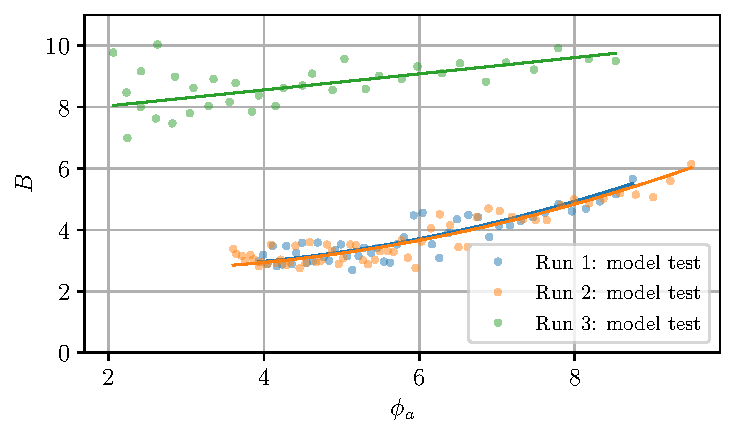
\includegraphics[width = 0.475\textwidth]{figures/mdl.pdf}\end{center}
\vspace{-0.7cm}
\caption{Model test roll damping}
\label{fig:mdl}
\end{figure}
\subsection*{Damping by Ikeda's method}\label{damping-by-ikedas-method}
Roll damping has been calculated for the validation cases with two
alternative implementations of Ikeda's method. The first alternative
uses the original semi-empirical formula to calculate $C_r$
coefficient for eddy damping. The second alternative uses the developed
decision tree. These two implementations of Ikeda's method are compared
with the corresponding model tests at 0 speed in
Fig.\ref{fig:ikeda} and at speed ($F_n=0.14)$ in
Fig.\ref{fig:ikeda_speed}. The left plots in these figures show
original Ikeda's method and the right plots show the decision tree
alternative. The decision tree alternative shows good agreement with the
model test for the 0 speed case. Ikeda's method gives much higher values
for this case. For the speed case, Ikeda's method has the best agreement
with model test. The decision tree alternative gives a damping that is
somewhat lower than the model test.
\begin{figure}[H]
\begin{center}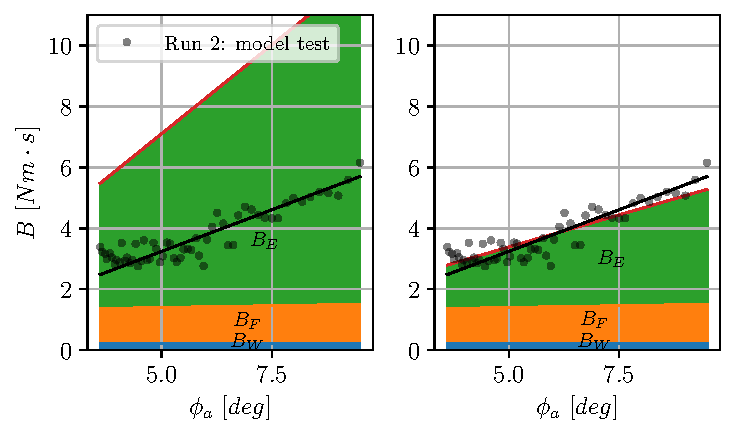
\includegraphics[width = 0.475\textwidth]{figures/ikeda.pdf}\end{center}
\vspace{-0.7cm}
\caption{Roll damping components calculated at zero speed with two alternative implementations of Ikeda's method: Regular implementation (left), Decision tree $C_r$ (right).}
\label{fig:ikeda}
\end{figure}
\begin{figure}[H]
\begin{center}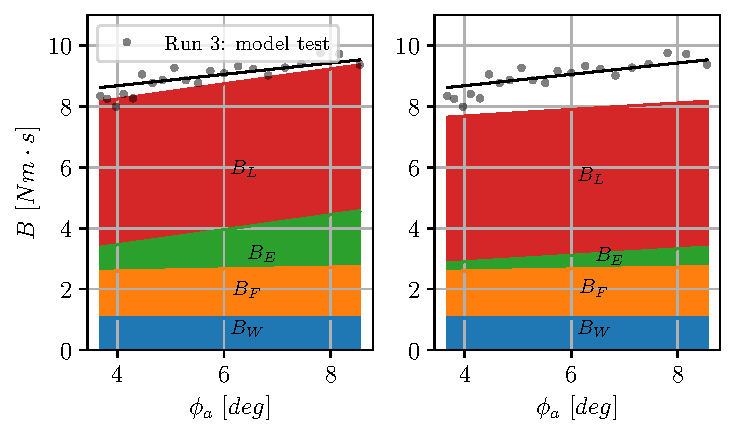
\includegraphics[width = 0.475\textwidth]{figures/ikeda_speed.pdf}\end{center}
\vspace{-0.7cm}
\caption{Roll damping components calculated at speed with two alternative implementations of Ikeda's method: Regular implementation (left), Decision tree $C_r$ (right).}
\label{fig:ikeda_speed}
\end{figure}
The $C_r$ coefficient has been calculated for KVLCC2 with section data
according to Tab.\ref{tab:kvlcc2_section_table}. A section wise
comparison between the two alternatives of Ikeda's method is shown in
Fig.\ref{fig:kvlcc2_eddy} where the regular implementation of
Ikeda's method predicts much higher $C_r$ between station 8 and 14.
These stations have almost rectangular shape (see
Fig.\ref{fig:body_plan}) with very small bilge radiuses
($R_b$). A small deviation of the sectional shape will have a large
impact on the eddy damping for this kind of sections. This can be seen
from the cylinder experiments in Fig.\ref{fig:ikeda_sections}
and also in the illustration in Fig.\ref{fig:kvlcc2_eddy}. The
decision tree and Ikeda's method capture this very nonlinear behaviour
differently, giving the deviating $C_r$ predictions for stations 8 to
14.
\begin{figure}[H]
\begin{center}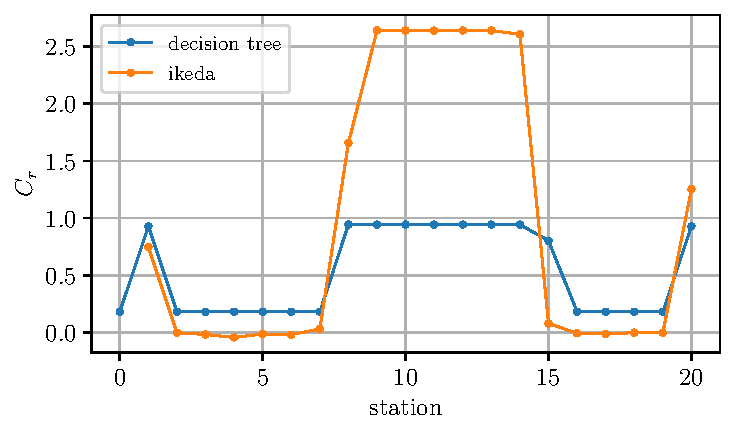
\includegraphics[width = 0.475\textwidth]{figures/kvlcc2_eddy.pdf}\end{center}
\vspace{-0.7cm}
\caption{KVLCC2 eddy damping coefficient along the hull}
\label{fig:kvlcc2_eddy}
\end{figure}
\subsection*{Motions estimated by FNPF}\label{motions-estimated-by-fnpf}
Simulations of roll decay tests were conducted with FNPF without viscous
damping. Wave damping obtained from these tests are shown in
Fig.\ref{fig:fnpf}. FNPF predicts higher wave damping for both 0
speed and at speed, compared to Ikeda's method (see
Fig.\ref{fig:ikeda} and Fig.\ref{fig:ikeda_speed}). The
FNPF wave damping does not change much with the roll amplitude which
means that it is reasonably linear. This confirms the assumption used in
the derivation of the eddy damping \citep{7505983/4AFVVGNT}.
\begin{figure}[H]
\begin{center}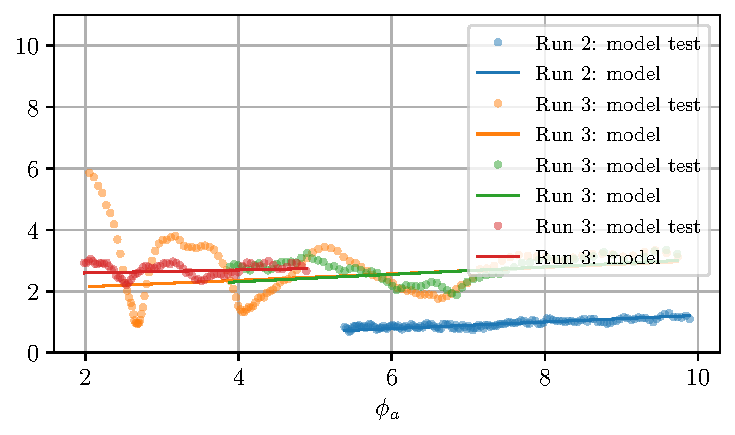
\includegraphics[width = 0.475\textwidth]{figures/fnpf.pdf}\end{center}
\vspace{-0.7cm}
\caption{Wave damping obtained from FNPF}
\label{fig:fnpf}
\end{figure}
\subsection*{Roll motion prediction with hybrid
method}\label{roll-motion-prediction-with-hybrid-method}
The hybrid method uses the decision tree in the calculation of eddy
damping and FNPF in the calculation of the wave damping.
Fig.\ref{fig:hybrid_0} and Fig.\ref{fig:hybrid_speed}
show comparisons between roll damping predicted with hybrid method and
model tests. The hybrid method predicts higher damping than the decision
tree alternative of Ikeda's method (see right plots in
Fig.\ref{fig:ikeda} and Fig.\ref{fig:ikeda_speed}) due
to the higher wave damping of FNPF. The hybrid method predicts roll
damping that is slightly higher than the model test for the 0 speed case
and very good agreement at speed case.
\begin{figure}[H]
\begin{center}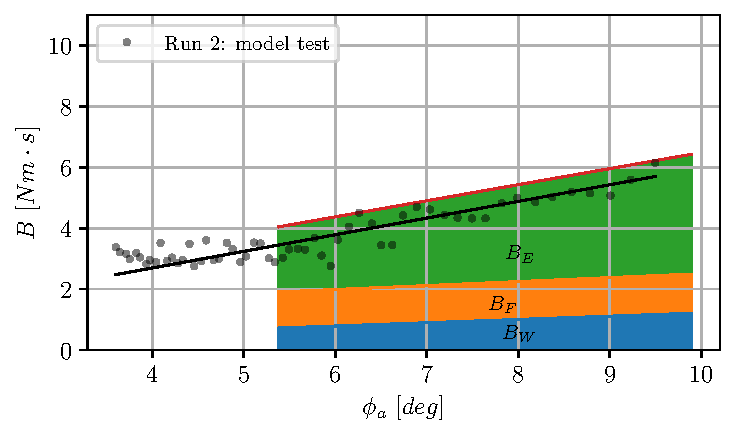
\includegraphics[width = 0.475\textwidth]{figures/hybrid_0.pdf}\end{center}
\vspace{-0.7cm}
\caption{Roll damping from hybrid method ($F_n = 0$)}
\label{fig:hybrid_0}
\end{figure}
\begin{figure}[H]
\begin{center}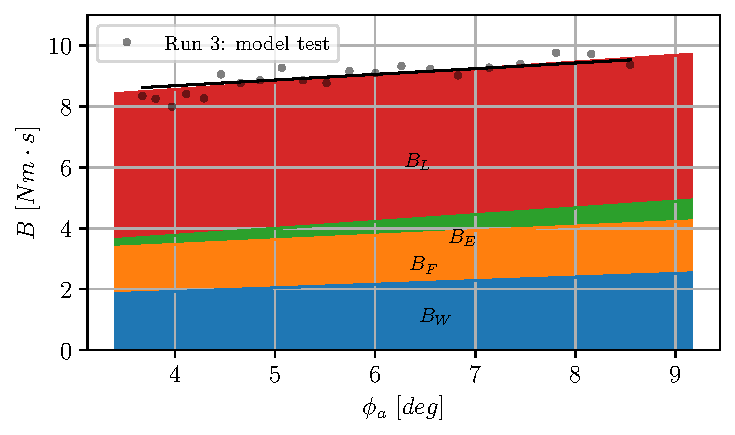
\includegraphics[width = 0.475\textwidth]{figures/hybrid_speed.pdf}\end{center}
\vspace{-0.7cm}
\caption{Roll damping from hybrid method ($F_n = 0.14$)}
\label{fig:hybrid_speed}
\end{figure}
The hybrid method can also be compared with the model tests in the time
domain. Time step simulations (see section "\nameref{se:pit}") with
damping coefficients from the hybrid method can be conducted to obtain
these predictions. Fig.\ref{fig:hybrid_0_time} shows a
comparison at 0 speed and Fig.\ref{fig:hybrid_speed_time} shows
a comparison at speed. The time series from the corresponding FNPF
simulations has also been added to these plots to show how much the
injection of semi-empirical viscous damping can improve the accuracy of
these simulations.
\begin{figure}[H]
\begin{center}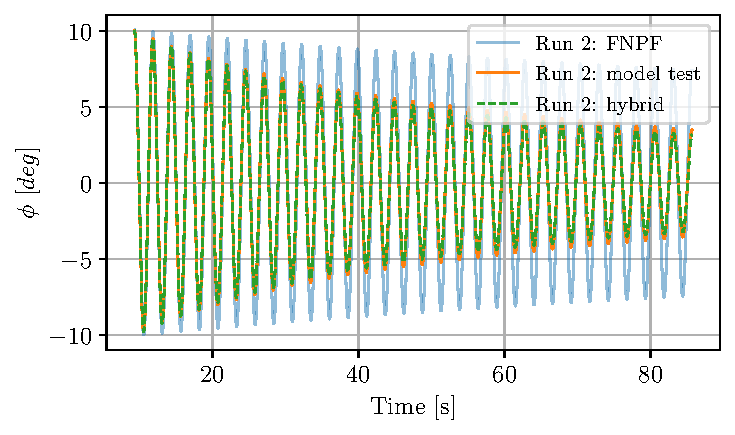
\includegraphics[width = 0.475\textwidth]{figures/hybrid_0_time.pdf}\end{center}
\vspace{-0.7cm}
\caption{Roll decay (0 kn)}
\label{fig:hybrid_0_time}
\end{figure}
\begin{figure}[H]
\begin{center}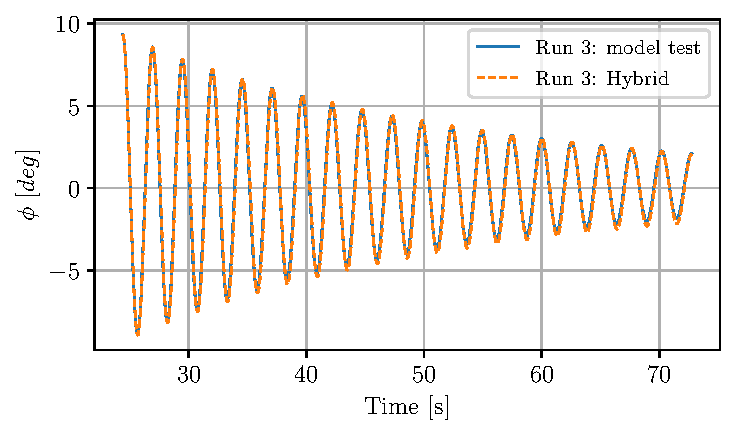
\includegraphics[width = 0.475\textwidth]{figures/hybrid_speed_time.pdf}\end{center}
\vspace{-0.7cm}
\caption{Roll decay (15.5 kn)}
\label{fig:hybrid_speed_time}
\end{figure}
The coefficients obtained from model tests, FNPF and hybrid method are
summarized in model scale units in the table below. The equivalent
linearized damping for 5 degrees roll angle amplitude $B_{e5}$ has
also been added to this table. It can be seen that the hybrid method
overpredicts the damping at 0 knots for this amplitude.
\begin{table}[H]
\scriptsize
\center
\caption{Roll damping coefficients for model scale KVLCC2}
\label{tab:results}
\begin{tabular}{|l|l|l|l|l|l|}
\hline\addlinespace
$F_n$ & run & method & $B_1$ & $B_2$ & $B_{e5}$\\
$[-]$ &  &  & $[Nm \cdot s]$ & $[Nm \cdot s^2]$ & $[Nm \cdot s]$\\
\hline0.0 & 1 & model test & 0.54 & 14.95 & 3.26\\
0.0 & 2 & model test & 0.51 & 14.98 & 3.24\\
0.0 & 2 & hybrid & 1.2 & 14.5 & 3.84\\
0.14 & 3 & model test & 7.93 & 5.1 & 8.87\\
0.14 & 3 & hybrid & 7.52 & 6.01 & 8.61\\
\hline
\end{tabular}
\end{table}
